% Options for packages loaded elsewhere
\PassOptionsToPackage{unicode}{hyperref}
\PassOptionsToPackage{hyphens}{url}
%
\documentclass[
]{article}
\usepackage{amsmath,amssymb}
\usepackage{iftex}
\ifPDFTeX
  \usepackage[T1]{fontenc}
  \usepackage[utf8]{inputenc}
  \usepackage{textcomp} % provide euro and other symbols
\else % if luatex or xetex
  \usepackage{unicode-math} % this also loads fontspec
  \defaultfontfeatures{Scale=MatchLowercase}
  \defaultfontfeatures[\rmfamily]{Ligatures=TeX,Scale=1}
\fi
\usepackage{lmodern}
\ifPDFTeX\else
  % xetex/luatex font selection
\fi
% Use upquote if available, for straight quotes in verbatim environments
\IfFileExists{upquote.sty}{\usepackage{upquote}}{}
\IfFileExists{microtype.sty}{% use microtype if available
  \usepackage[]{microtype}
  \UseMicrotypeSet[protrusion]{basicmath} % disable protrusion for tt fonts
}{}
\makeatletter
\@ifundefined{KOMAClassName}{% if non-KOMA class
  \IfFileExists{parskip.sty}{%
    \usepackage{parskip}
  }{% else
    \setlength{\parindent}{0pt}
    \setlength{\parskip}{6pt plus 2pt minus 1pt}}
}{% if KOMA class
  \KOMAoptions{parskip=half}}
\makeatother
\usepackage{xcolor}
\usepackage[margin=1in]{geometry}
\usepackage{longtable,booktabs,array}
\usepackage{calc} % for calculating minipage widths
% Correct order of tables after \paragraph or \subparagraph
\usepackage{etoolbox}
\makeatletter
\patchcmd\longtable{\par}{\if@noskipsec\mbox{}\fi\par}{}{}
\makeatother
% Allow footnotes in longtable head/foot
\IfFileExists{footnotehyper.sty}{\usepackage{footnotehyper}}{\usepackage{footnote}}
\makesavenoteenv{longtable}
\usepackage{graphicx}
\makeatletter
\def\maxwidth{\ifdim\Gin@nat@width>\linewidth\linewidth\else\Gin@nat@width\fi}
\def\maxheight{\ifdim\Gin@nat@height>\textheight\textheight\else\Gin@nat@height\fi}
\makeatother
% Scale images if necessary, so that they will not overflow the page
% margins by default, and it is still possible to overwrite the defaults
% using explicit options in \includegraphics[width, height, ...]{}
\setkeys{Gin}{width=\maxwidth,height=\maxheight,keepaspectratio}
% Set default figure placement to htbp
\makeatletter
\def\fps@figure{htbp}
\makeatother
\setlength{\emergencystretch}{3em} % prevent overfull lines
\providecommand{\tightlist}{%
  \setlength{\itemsep}{0pt}\setlength{\parskip}{0pt}}
\setcounter{secnumdepth}{-\maxdimen} % remove section numbering
% definitions for citeproc citations
\NewDocumentCommand\citeproctext{}{}
\NewDocumentCommand\citeproc{mm}{%
  \begingroup\def\citeproctext{#2}\cite{#1}\endgroup}
\makeatletter
 % allow citations to break across lines
 \let\@cite@ofmt\@firstofone
 % avoid brackets around text for \cite:
 \def\@biblabel#1{}
 \def\@cite#1#2{{#1\if@tempswa , #2\fi}}
\makeatother
\newlength{\cslhangindent}
\setlength{\cslhangindent}{1.5em}
\newlength{\csllabelwidth}
\setlength{\csllabelwidth}{3em}
\newenvironment{CSLReferences}[2] % #1 hanging-indent, #2 entry-spacing
 {\begin{list}{}{%
  \setlength{\itemindent}{0pt}
  \setlength{\leftmargin}{0pt}
  \setlength{\parsep}{0pt}
  % turn on hanging indent if param 1 is 1
  \ifodd #1
   \setlength{\leftmargin}{\cslhangindent}
   \setlength{\itemindent}{-1\cslhangindent}
  \fi
  % set entry spacing
  \setlength{\itemsep}{#2\baselineskip}}}
 {\end{list}}
\usepackage{calc}
\newcommand{\CSLBlock}[1]{\hfill\break\parbox[t]{\linewidth}{\strut\ignorespaces#1\strut}}
\newcommand{\CSLLeftMargin}[1]{\parbox[t]{\csllabelwidth}{\strut#1\strut}}
\newcommand{\CSLRightInline}[1]{\parbox[t]{\linewidth - \csllabelwidth}{\strut#1\strut}}
\newcommand{\CSLIndent}[1]{\hspace{\cslhangindent}#1}
\usepackage{float}
\ifLuaTeX
  \usepackage{selnolig}  % disable illegal ligatures
\fi
\usepackage{bookmark}
\IfFileExists{xurl.sty}{\usepackage{xurl}}{} % add URL line breaks if available
\urlstyle{same}
\hypersetup{
  pdftitle={Homework 2 Solutions},
  hidelinks,
  pdfcreator={LaTeX via pandoc}}

\title{Homework 2 Solutions}
\author{}
\date{\vspace{-2.5em}}

\begin{document}
\maketitle

\(\bf (1)\) Rocket League is a popular online video game and E-sport
that emerged in 2015. The game enjoys a healthy following of around 93
million players per month. The game features players from around the
world who compete in sports like soccer (football), basketball and
hockey while controlling RC-like vehicles. The most popular game-mode is
doubles soccer in which teams of two players each try to outscore each
other by hitting a soccer ball into the opposing goal. In the course of
each match, the player-controlled vehicles often collide in what is
commonly referred to as a ``bump''. The following histogram shows the
distribution of the average number of ``bumps'' per match for a given
player of Rocket League


\includegraphics{week5homework_solns_files/figure-latex/unnamed-chunk-1-1.pdf}

\begin{enumerate}
\def\labelenumi{(\alph{enumi})}
\tightlist
\item
  Assuming a mean of \(\bar{x} = 355\) and standard deviation of
  \(s = 69\), in approximately what proportion of matches did the player
  have more than 423 bumps?
\end{enumerate}

{\[ z = \frac{423 - 355}{69} \approx 1\]. Therefore we want to know what
proportion of observations have a value \(\geq \bar{x}+1s\) which is by
the empirical rule is \(13.5\%+2.5\% = 16\%\)}

\begin{enumerate}
\def\labelenumi{(\alph{enumi})}
\setcounter{enumi}{1}
\tightlist
\item
  Approximately what proportion of matches did the player have more than
  217 bumps but fewer than 493 bumps?
\end{enumerate}

{approximately \(95\%\)}

\begin{enumerate}
\def\labelenumi{(\alph{enumi})}
\setcounter{enumi}{2}
\tightlist
\item
  How many bumps would the player need to have in a match to be in the
  top \(2.5\%\) of matches?
\end{enumerate}

{at least \(355+2s = 493\) bumps}

\begin{enumerate}
\def\labelenumi{(\alph{enumi})}
\setcounter{enumi}{3}
\tightlist
\item
  After playing a new match, the player logs 620 bumps. Calculate the
  \(z\)-score for this match and explain the meaning of the z-score in
  relation to the average number of bumps. How many standard deviations
  is the player's performance from the mean number of bumps?
\end{enumerate}

{\[ z = \frac{620 - 355}{69} = 3.84 \] The player's performance in this
match is \(3.84\) standard deviations \textbf{above} the mean number of
bumps. A \(z\)-score this large means the match is extremely unusual for
this player - under the empirical rule almost all matches fall within
\(3\) standard deviations of the mean, so 620 bumps is far beyond the
player's typical performance.}

\begin{longtable}[]{@{}
  >{\centering\arraybackslash}p{(\columnwidth - 2\tabcolsep) * \real{0.5000}}
  >{\centering\arraybackslash}p{(\columnwidth - 2\tabcolsep) * \real{0.5000}}@{}}
\toprule\noalign{}
\begin{minipage}[b]{\linewidth}\centering
\textbf{Figure 1} Pinniped whisker morphology - Ginter et al.~2012
\end{minipage} & \begin{minipage}[b]{\linewidth}\centering
A juvenile Harp Seal
\end{minipage} \\
\midrule\noalign{}
\endhead
\bottomrule\noalign{}
\endlastfoot
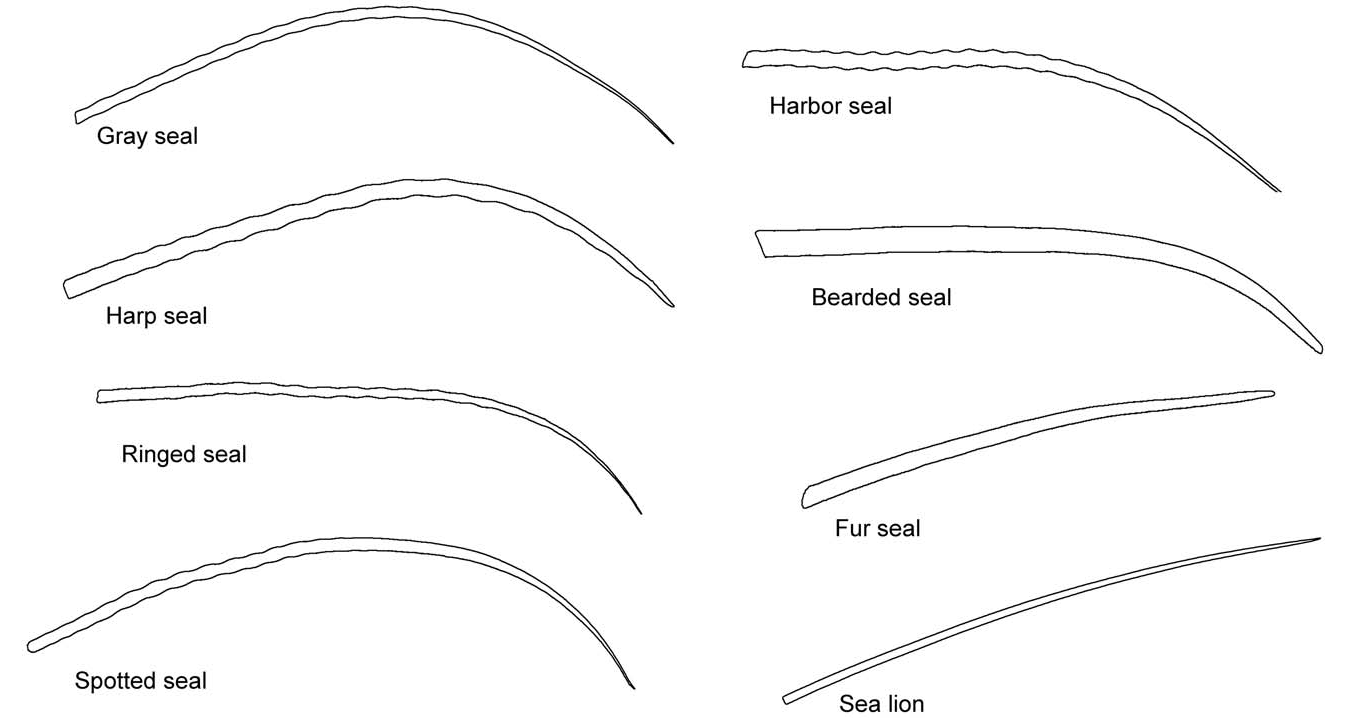
\includegraphics{../assets/whisker_types.png} &
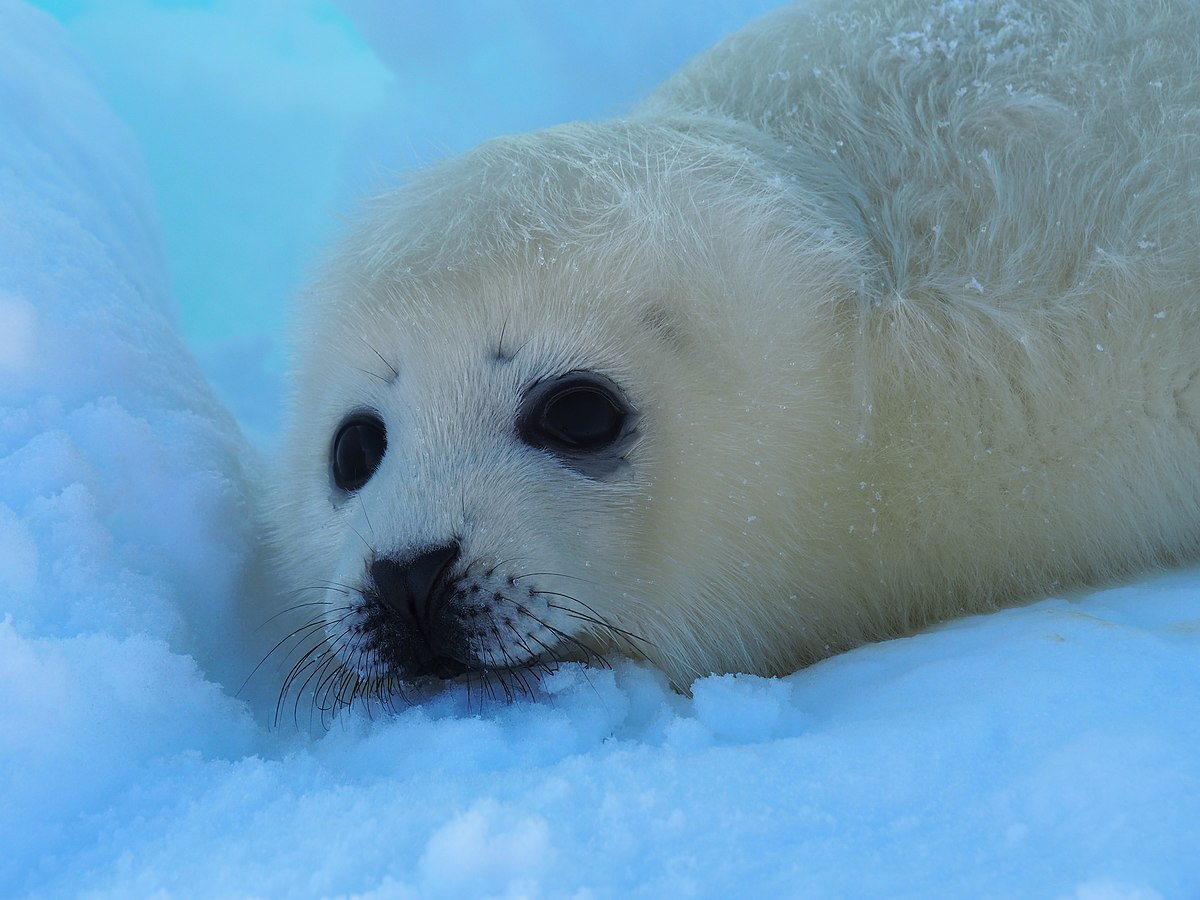
\includegraphics{../assets/Harp_seal_whitecoat.jpg} \\
\end{longtable}

\(\bf (2)\) Pinnipeds (seals and sea lions) possess the largest
vibrissae (whiskers) among mammals and their vibrissal hair shafts
demonstrate a diversity of shapes (\textbf{See Figure 1}). In a study
conducted by (Ginter et al. 2012), researchers measured 9
characteristics of Pinniped whiskers in individuals from 9 species of
seals and sea lions. Their goal was to better characterize whisker
morphology and evolution. The following data are the recorded whisker
lengths of 20 Harp Seals (given in \textbf{Table 1}). Note that the data
have been sorted according to increasing ``Total Length (cm)'' for your
convenience - use the table to answer the following questions:

\newpage

\begin{table}[H]
\centering\centering
\caption{\label{tab:unnamed-chunk-3}Whisker Length data for $n = 20$ Harp Seals}
\centering
\begin{tabular}[t]{rrr}
\toprule
Observation & Whisker Total Length (cm) & Number of Beads\\
\midrule
\cellcolor{gray!10}{1} & \cellcolor{gray!10}{4.18} & \cellcolor{gray!10}{2}\\
2 & 4.23 & 2\\
\cellcolor{gray!10}{3} & \cellcolor{gray!10}{4.31} & \cellcolor{gray!10}{2}\\
4 & 4.31 & 2\\
\cellcolor{gray!10}{5} & \cellcolor{gray!10}{4.33} & \cellcolor{gray!10}{2}\\
\addlinespace
6 & 4.34 & 2\\
\cellcolor{gray!10}{7} & \cellcolor{gray!10}{4.35} & \cellcolor{gray!10}{2}\\
8 & 4.38 & 2\\
\cellcolor{gray!10}{9} & \cellcolor{gray!10}{4.40} & \cellcolor{gray!10}{2}\\
10 & 4.41 & 2\\
\addlinespace
\cellcolor{gray!10}{11} & \cellcolor{gray!10}{4.43} & \cellcolor{gray!10}{3}\\
12 & 4.44 & 2\\
\cellcolor{gray!10}{13} & \cellcolor{gray!10}{4.46} & \cellcolor{gray!10}{2}\\
14 & 4.47 & 3\\
\cellcolor{gray!10}{15} & \cellcolor{gray!10}{4.48} & \cellcolor{gray!10}{3}\\
\addlinespace
16 & 4.51 & 2\\
\cellcolor{gray!10}{17} & \cellcolor{gray!10}{4.59} & \cellcolor{gray!10}{3}\\
18 & 4.60 & 2\\
\cellcolor{gray!10}{19} & \cellcolor{gray!10}{4.62} & \cellcolor{gray!10}{2}\\
20 & 5.08 & 3\\
\bottomrule
\end{tabular}
\end{table}

\begin{verbatim}
## [1] "comma separated values = 4.18,4.23,4.31,4.31,4.33,4.34,4.35,4.38,4.4,4.41,4.43,4.44,4.46,4.47,4.48,4.51,4.59,4.6,4.62,5.08"
\end{verbatim}

\newpage

\begin{enumerate}
\def\labelenumi{(\alph{enumi})}
\tightlist
\item
  Compute the quartiles, interquartile range, mean, and standard
  deviation for the variable ``Total Length (cm)'' - (use the course
  website apps for help)
\end{enumerate}

{\begin{eqnarray} Q1 = \frac{4.33+4.34}{2} = 4.335 \approx 4.34 \\\nonumber
 median =  \frac{4.41+4.43}{2} = 4.42 \\\nonumber
 Q3 = \frac{4.48+4.51}{2} = 4.49 \\\nonumber
 IQR =  4.49 - 4.34 = 0.15 \\\nonumber
 \bar{x} =  \frac{4.18 + 4.23 + \cdots + 5.08}{20} = 4.446 \\\nonumber
 s =  \sqrt{\frac{(4.18 - 4.45)^2 + (4.23 - 4.45)^2 + \cdots + (5.08 - 4.45)^2}{19}} = 0.189 \\\nonumber
\end{eqnarray}}

\begin{enumerate}
\def\labelenumi{(\alph{enumi})}
\setcounter{enumi}{1}
\tightlist
\item
  Make a boxplot of the variable ``Total Length'' and make note of any
  outliers
\end{enumerate}


\includegraphics{week5homework_solns_files/figure-latex/unnamed-chunk-4-1.pdf}

\begin{enumerate}
\def\labelenumi{(\alph{enumi})}
\setcounter{enumi}{2}
\tightlist
\item
  Observation 20 has a total whisker length of 5.08 (cm), how many
  standard deviations is this observation from the mean whisker length?
  (hint compute the \(z\)-score for this observation)
\end{enumerate}

{The sample mean is \(\bar{x} = 4.446\) and the sample standard
deviation is \(s = 0.189\)
\[ z = \frac{5.08 - \bar{x}}{s} = \frac{5.080 - 4.446}{0.189} = 3.372  \]}

\(\bf (3)\) Use the following pair of boxplots constructed from the
Pinniped whisker data in \(\textbf{Table 1}\). The boxplots show the
distribution of total whisker length (cm) for whiskers with 2 beads vs
whiskers with three beads. Answer the following questions:


\includegraphics{week5homework_solns_files/figure-latex/unnamed-chunk-5-1.pdf}

\begin{verbatim}
## [1] "-----------------2 bead whisker lengths-----------------"
\end{verbatim}

\begin{verbatim}
## [1] "comma separated values =  4.3,4.6,4.5,4.6,4.2,4.3,4.3,4.2,4.4,4.3,4.5,4.3,4.4,4.4,4.4"
\end{verbatim}

\begin{verbatim}
## [1] "-----------------3 bead whisker lengths-----------------"
\end{verbatim}

\begin{verbatim}
## [1] "comma separated values =  4.6,5.1,4.5,4.4,4.5"
\end{verbatim}

\begin{enumerate}
\def\labelenumi{(\alph{enumi})}
\tightlist
\item
  Using the boxplot above, do the whisker lengths for 2 bead and 3 bead
  whiskers follow a normal distribution? why or why not?
\end{enumerate}

{The boxplot for 2 bead whiskers is roughly symmetric, which is
consistent with (though not proof of) an approximately normal
distribution. The boxplot for 3 bead whiskers is clearly skewed, so
those whisker lengths are not approximately normal}

\begin{enumerate}
\def\labelenumi{(\alph{enumi})}
\setcounter{enumi}{1}
\tightlist
\item
  Suppose researchers observe two new Harp Seals (Denoted Seal 1 and
  Seal 2) and record their total whiskers lengths and the number of
  beads on the whiskers. Seal 1 has a total whisker length of 4.32 (cm)
  and the whisker has 3 beads. Seal 2 has a total whisker length of 4.34
  (cm) but the whisker has only 2 beads. Suppose we want to know how
  they compare relative to the distribution of whiskers with the same
  number of beads. Confirm that the whisker length of seal 1 has a
  \(z\)-score of \(-1.07\) while Seal 2 has a \(z\)-score of \(-0.43\).
  Refer to the boxplot above
\end{enumerate}

{The mean length for whiskers with two beads and three beads is
\(\bar{x}_{2beads} = 4.39\) and \(\bar{x}_{3beads} = 4.61\)
respectively. The standard deviation in length for whiskers with 2 and 3
beads is \(s_{2beads} = 0.121\) and \(s_{3beads} = 0.270\) respectively.
Seal 1 has a \(z\)-score of
\[z_1 = \frac{4.32 - \bar{x_3}}{s_3} = \frac{4.32 - 4.61}{0.27} = -1.07\]
And Seal 2 has a \(z\)-score of
\[z_2 = \frac{4.34 - \bar{x_2}}{s_2} = \frac{4.34 - 4.39}{0.12} = -0.43\]
}

\begin{enumerate}
\def\labelenumi{(\alph{enumi})}
\setcounter{enumi}{2}
\tightlist
\item
  If the researchers were to observe the whisker length of a new seal
  and the whisker had 3 beads, how long or short would the whisker of
  this observation have to be for it to be considered an outlier?
  (assume the data is approximately normal)
\end{enumerate}

{Since the data is approximately symmetric (normal) we can use the 2
standard deviations rule: an observation is flagged as an outlier when
\(x < \bar{x}-2s\) \textbf{or} \(x > \bar{x}+2s\) - so the whisker would
have to be greater than
\[ \bar{x}_3 + 2s = 4.608 + 2\times 0.270 = 5.148 (cm) \] or less than
\[ \bar{x}_3 - 2s = 4.608 - 2\times 0.270 = 4.068 (cm)\]}

\(\bf (4)\) Use the following plot of the cumulative distribution of a
quantitative variable \(x\) to answer questions (a)-(c)


\includegraphics{week5homework_solns_files/figure-latex/unnamed-chunk-6-1.pdf}

\begin{verbatim}
## [1] "Comma separated values =  -4.7,-2.5,-2.3,-1.3,-1.3,-1.2,0,0,1,1.8,2.1,2.3,2.6,2.8,2.8,2.9,3.5,3.6,3.7,3.7,4.3,4.8,4.9,5.2,5.3,5.5,6,6.5,6.6,7.1,7.1,7.2,7.4,7.7,7.8,8.1,8.1,8.1,8.5,8.7,9,9,10,10.2,10.2,11,11,11.1,11.1,11.5"
\end{verbatim}

\begin{enumerate}
\def\labelenumi{(\alph{enumi})}
\tightlist
\item
  Assume that the mean and standard deviation of \(X\) are
  \(\bar{x} = 5\) and \(s = 4\). Use these values to find the \(2.5th\)
  and \(97.5th\) percentiles of \(X\). Compare your answer with the
  cumulative distribution plot above, why might the two answers differ?
  (hint: think about shape and how that relates to the empirical rule)
\end{enumerate}

{approximately \(-3\) and \(13\). Using the plot above the answers are
approximately -2.5 and 11.1. The percentiles differ because the
distribution of \(X\) is skewed to the left. The percentiles given by
the empirical rule are only approximate for distributions with
deviations from normality}

\begin{enumerate}
\def\labelenumi{(\alph{enumi})}
\setcounter{enumi}{1}
\tightlist
\item
  Assume the above cumulative distribution represents an approximately
  normal distribution (symmetric, bell-shaped) with a standard deviation
  of \(s = 4\) and a mean of \(\bar{x} = 5\), Under the empirical rule,
  what percentage of the observations will have a value between \(-3\)
  and \(13\)?
\end{enumerate}

{if the mean is \(\bar{x} = 5\) then both \(-3\) and \(13\) are two
standard deviations from the mean e.g \(-3 = \bar{x}-2s\) and
\(13 = \bar{x}+2s\). Under the empirical rule, appoximately \(95\%\) of
the observations will fall in this interval }

\begin{enumerate}
\def\labelenumi{(\alph{enumi})}
\setcounter{enumi}{2}
\tightlist
\item
  Using the mean and standard deviation from part a-b, compute and
  interpret the z-scores for the observations \(x_1 = 11.5\) and
  \(x_2 = -4.7\). Would these two observations be considered outliers
  under the \(\pm 2s\) rule?
\end{enumerate}

{ \[ z_1 = \frac{11.5 - 5}{4} \approx 1.63 \] The observation
\(x_1 = 11.5\) sits \(1.63\) standard deviations above the mean. It is
not an outlier, because \(1.63 < 2\) } {
\[ z_2 = \frac{-4.7 - 5}{4} \approx -2.43 \] The observation
\(x_2 = -4.7\) sits \(2.43\) standard deviations below the mean. It
would be flagged as an outlier, because \(-2.43 < -2\) }

\(\bf (5)\) Define the following terms

\begin{enumerate}
\def\labelenumi{(\alph{enumi})}
\item
  Explanatory variable - {The independent variable which we manipulate
  to see how the response variable changes}
\item
  Response variable - {The outcome or dependent variable - the variable
  on which we make comparisons for different values of the explanatory
  variable }
\item
  experimental study - {A study which assigns subjects/observations to
  one or more treatments and observes the outcome of the response
  variable }
\item
  observational study - {A nonexperimental study in which the researcher
  observes values of the response and explanatory variables for each
  subject/observation}
\item
  survey - {A type of nonexperimental study in which
  subjects/observations are selected from a population for the purpose
  of making inferences about the population.}
\end{enumerate}

\(\bf (6)\) Name the sampling method used in each of the following
situations:

\begin{enumerate}
\def\labelenumi{(\alph{enumi})}
\tightlist
\item
  A man is standing outside of a grocery store handing out
  questionnaires to shoppers asking them to evaluate their shopping
  experience and the quality of service. He does not ask shoppers who
  have their hands full carrying groceries, but instead asks all
  shoppers who have only a few items or have both hands free to fill out
  the questionnaire.
\end{enumerate}

{convenience sampling}

\begin{enumerate}
\def\labelenumi{(\alph{enumi})}
\setcounter{enumi}{1}
\tightlist
\item
  A gardener has a garden box in which he has planted 10 rows of corn.
  Each row consists of eight corn plants. The gardener wishes to know
  the average height of the corn plants in the garden box so he randomly
  selects rows 1, 5, and 9 and measures the height of all corn plants in
  those rows.
\end{enumerate}

{cluster sampling}

\begin{enumerate}
\def\labelenumi{(\alph{enumi})}
\setcounter{enumi}{2}
\tightlist
\item
  A company wishes to know how employees feel about compensation and
  benefits. Over the next few weeks, the company asks 30 employees from
  each of its branch locations to fill out a survey regarding
  compensation.
\end{enumerate}

{stratified random sampling}

\begin{enumerate}
\def\labelenumi{(\alph{enumi})}
\setcounter{enumi}{3}
\tightlist
\item
  A local polling company wishes to know what proportion of citizens in
  Moscow, Idaho are voting for the Republican candidate in the mayoral
  race. The polling company records this information for every 5th voter
  who leaves the voting booth.
\end{enumerate}

{systematic sampling}

\begin{enumerate}
\def\labelenumi{(\alph{enumi})}
\setcounter{enumi}{4}
\tightlist
\item
  A lumber company wishes to estimate the amount of usable lumber on a
  plot of land. The company randomly selects 100 trees and measures
  their diameter, height, and volume, in order to estimate the number of
  board feet of each tree.
\end{enumerate}

{simple random sampling}

\newpage

\section{References}\label{references}

\newpage
\section{References}

\phantomsection\label{refs}
\begin{CSLReferences}{1}{0}
\bibitem[\citeproctext]{ref-ginter2012fused}
Ginter, Carly C, Thomas J DeWitt, Frank E Fish, and Christopher D
Marshall. 2012. {``Fused Traditional and Geometric Morphometrics
Demonstrate Pinniped Whisker Diversity.''} \emph{PloS One} 7 (4):
e34481.

\end{CSLReferences}

\end{document}
